% Please compile the tex file by pdfLaTeX, 
% it would handle the landscape pages correctly.
\documentclass[12pt]{mines-thesis}
% Font Size: 10-12 point type, change the value above

%========================================
%                              Set-up                              
%========================================
% Text will be double spaced or 1.5 spaced. 
%\OnehalfSpacing 
\DoubleSpacing
% Set the indentation of each paragraph.
\setlength{\parindent}{2em}
% Set the lowest level to show in the table of contents
\maxtocdepth{subsubsection}
% Set the fully-justified or left-justified text
%\textalignment{fully-justified}
%\textalignment{left-justified}

%========================================
%                           Packages                             
%========================================
\usepackage{lipsum} % dummy text
\usepackage{graphicx} % for images
\usepackage{natbib} % for Chicago style references
% hyperref is a package that frequently requires compiling twice 
\usepackage{hyperref} % for \url and links 
\usepackage{pdflscape} % for landscape mode page
\usepackage{everypage} % for landscape mode page numbering 
\usepackage{longtable} % for really long tables

% Place all chapter tex files in ``Chapters'' folder
% Place all references bib files in ``References'' folder

% Place all figures in ``Figures'' folder
\graphicspath{{Figures/}} 
% Or define several directories to be searched for figures.
% \graphicspath{{Figures/}{../figures/}{C:/Users/me/Documents/project/figures/}}


\begin{document}
%========================================
%                            Front Matter                              
%========================================
\autotitle %automatically change the title into upper cases and reshape it to an inverted pyramid
%\title{Thesis title centered on the page vertically and horizontally, in all upper case letters and in an inverted pyramid shape. Math mode: $\frac{2^{15}}{\pi}$}
% If you want to break the title by yourself, you must use ``\protect\\ ''.
% For example,
\title{
	Thesis title centered on the page vertically and horizontally, \protect\\
	in all upper case letters and in an inverted\protect\\
	pyramid shape. 	Math mode: $\frac{2^{15}}{\pi}$
}
	
\author{Student Name}  % this is your name exactly as you want it
\year{2020}     % this is the year of defence
\degree{Doctor of Philosophy}{Computer Science} %
\advisor{Dr. Thesis Advisor}
\coadvisor{Dr. Co-Advisor}  % comment out this line  if no co-advisor
\department{Department of XXX}
\departmenthead{Dr. Department Head}
	
	
%==================Abstracts===============
% 1. Are generally 200-300 words in length, 
% 2. Consist of one to two paragraphs of information,
% 3. Does not usually contain citations, 
% 4. Do not repeat the thesis title, and
% 5. Each paragraph should be indented.	
\begin{abstract}
	The abstract is a concise, one to three sentence statement of the thesis problem, a brief description consisting of no more than a few sentences describing the research method or design, and a report of the major findings and conclusions.
	%
			
	%
	The abstract submitted online at the time of thesis submission should be the same as the abstract inside the thesis. ProQuest continues to publish print indexes that have maximum abstract lengths of 150 words for Masters and 350 words for PhDs. Abstracts exceeding these limits will be truncated in the print indexes so it may be wise to work within those word limits in most cases.
\end{abstract}

%%============Acknowledgements==============
% Comment the section out if you don't need it 
%\begin{acknowledgment}
%	This optional page includes a paragraph or two acknowledging and thanking your
%	advisor(s), committee members, funding sponsors, family members etc.
%			
%	Typically, if you acknowledge everyone here, you won’t have a dedication page.
%	
%	Below are dummy texts generated  by the \texttt{lipsum} package.
%	\lipsum[3]
%\end{acknowledgment}

%%==================Dedication===============
% Comment the section out if you don't need it 
\begin{dedication}
	Dedication Page: A dedication page is optional and not frequently included in a thesis. However, occasionally the thesis writer wants to dedicate the document to a professional colleague, friend, or relative. A dedication typically expresses gratitude for someone's support. If a dedication page is included, it is placed at the end of the front matter section, following the acknowledgments. Typically, a dedication page has no title, it simply states, e.g., "For my father." Roman numeral page numbering continues on the dedication page.
\end{dedication}	


\makefrontmatter


%========================================
%                              Main Body                              
%========================================
%TODO Main Body
	
% You can separate the chapters to different files

%========================================
%                            Chapter                            
%======================================== 
\chapter{Introduction \protect\\ \NoCaseChange{This could be a subtitle}}
%TODO subtitle
\lipsum[2]

%========================================
%                            Section                             
%======================================== 	 
\section{First section}
\lipsum[3]

%========================================
%                            Section                             
%======================================== 
\section{Sencond  section}
\lipsum[3]
\subsection{First SubSection}
\lipsum[3]
\subsection{Second SubSection}
\lipsum[3]
\subsubsection{Sub SubSection}
\lipsum[3]	 
	 
%========================================
%                            Section                             
%======================================== 
\section{Last section Math mode: $\frac{2^{15}}{\pi}$} 
\lipsum[3]
\section{Last section to test Citation} 

First paper~\cite{goossens1994latex} did something. Note that here we use \verb|~| to make sure the citation not go to the other line. 

Lamport et al.~\cite{lamport1994latex} did something.

Many papers~\cite{makuuchi2000progress,yassin1994latex} did something.


All papers~\cite{makuuchi2000progress,yassin1994latex,
	goossens1994latex,lamport1994latex} did something.

Online link~\cite{onlineWindows} is about something.

More papers: \cite{colu92}, \cite{goossens1994latex}, \cite{jame76}, \cite{colu92,phil99,gree00,smit54}

%========================================
%                            Chapter                            
%======================================== 
\chapter{Reproduced Chapter:  This chapter represents that style used when a journal article has already been published or has been accepted for publication }
\reproduceinfo{
	Reproduced with permission from The Journal of Geology\\
	2012 Elsevier Ltd. 
	Katherine Smith\symbolfootnote{1}{Primary author and editor.}\footnote[1]{Department of  Civil and Environmental Engineering, Colorado School of Mines, 1500 Illinois Street, Golden, Colorado 80401, USA.}, 
	Eric Wright\symbolfootnote{2}{Corresponding author. Direct correspondence to \texttt{example@mines.edu}.}\footnote[2]{Southern Nevada, 550 City Parkway, Suite 810, Las Vegas, NV, 89106, USA.}
}
%\reproduceabstract % Print Abstract at the left




\section{Abstract}
This is the original abstract of your paper.This is the original abstract of your paper. This is the original abstract of your paper.This is the original abstract of your paper.

\lipsum[4]

%========================================
%                            Section                             
%======================================== 
\section{First section} 
\lipsum[2]

%========================================
%                            Chapter                            
%======================================== 
\chapter{This is a really really long title that someone else wrote for all the penguins in the world}
\lipsum[2]

%========================================
%                            Section                             
%======================================== 	
\section{First section}
\lipsum[3]

%========================================
%                            Section                             
%======================================== 
\section{This is a really really really really really really really really really really really really really really really really really really really really really really really really really really really really really really long title having more than three lines of text to appear on the toc.}
\lipsum[3-4]

%========================================
%                            Section                             
%======================================== 	 
\section{Last section} 
\lipsum[4]

%========================================
%                            Chapter                            
%======================================== 
\chapter{Example of Long  Long Long Long Long Long Long Long Long Long Long Long Long Long Long Long Long Long Long Long Long Long Long Long Long Long chapter}
\lipsum[4]
	
%========================================
%                            Section                             
%======================================== 	
\section{First section}
\lipsum[2]
\subsection{Subsection}
\lipsum[5]
\subsection{This is a really really really really really really really really really really really really really really really really really really really really really really really really really really really really really really long title having more than three lines of text to appear on the toc.}
\lipsum[4]
\subsubsection{SubSubsection}
\lipsum[5]

%========================================
%                            Section                             
%======================================== 
\section{Second section}
\lipsum[4]

%========================================
%                            Section                             
%======================================== 
\section{Last section} 
\lipsum[6]



%========================================
%              Chapter              
%======================================== 
\chapter{Figure and Table Chapter}
\lipsum[5]
%========================================
%              Section               
%======================================== 
\section{Figures}

The ``\verb|figure|'' environment should be used for figures. One or
more images can be placed within a figure. If your figure contains
third-party material, you must clearly identify it as such, as shown
in the example below.
\begin{figure}[h]
	\centering
	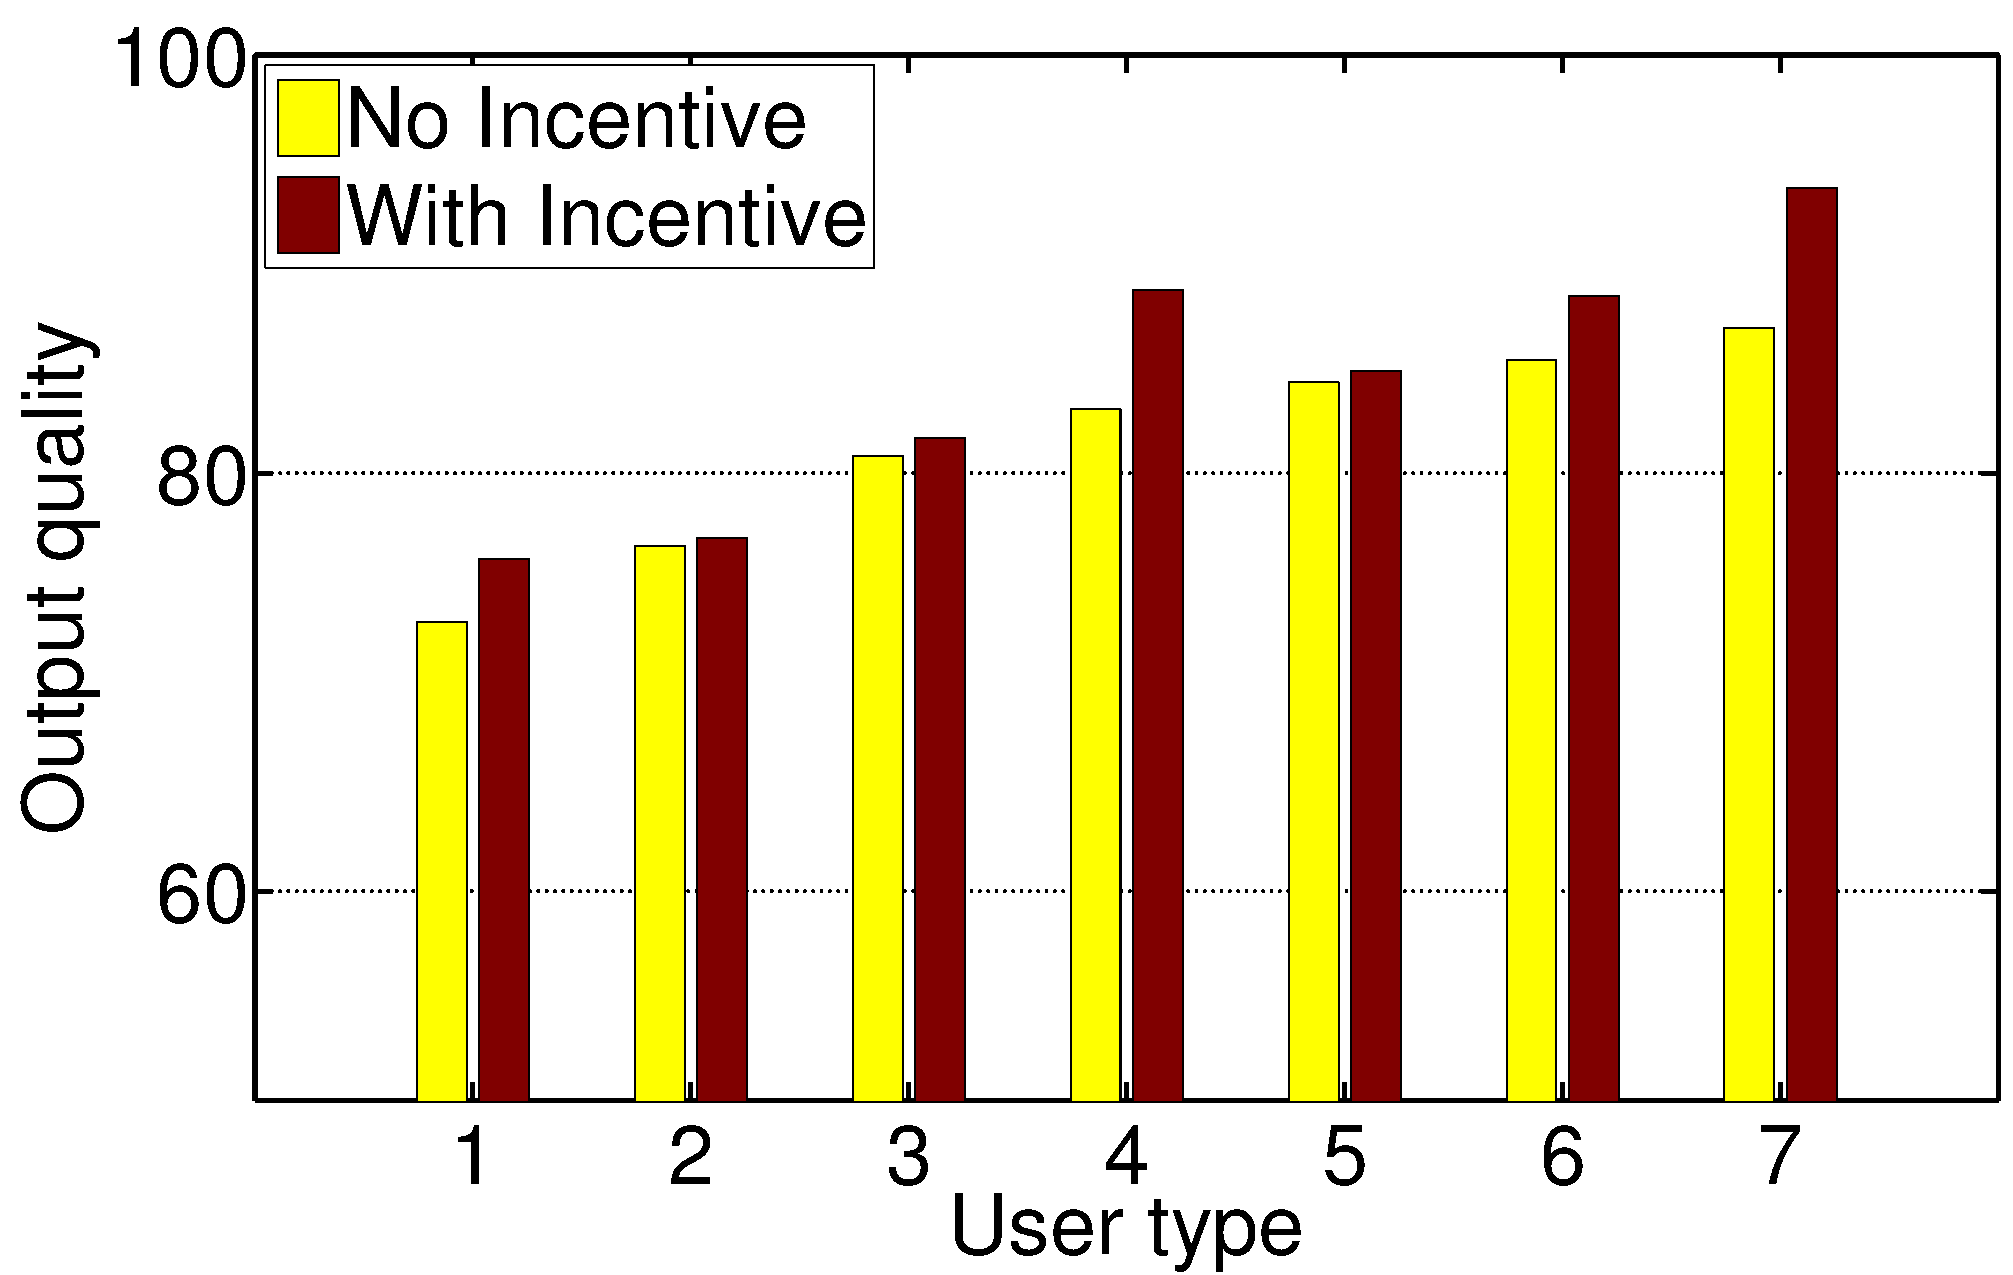
\includegraphics[width=\linewidth]{fig1}
	\caption{The figure with long long long long long long long long long long long long long long long long long long long long long long long long long long long long long long long long caption and links. (\url{https://goo.gl/VLCRBB}).}
\end{figure}



\lipsum[1-2]
\begin{landscape} % Require pdflscape and everypage packadge
	\begin{figure}[h]
		\centering
		% will generate blank page if use full  \linewidth
		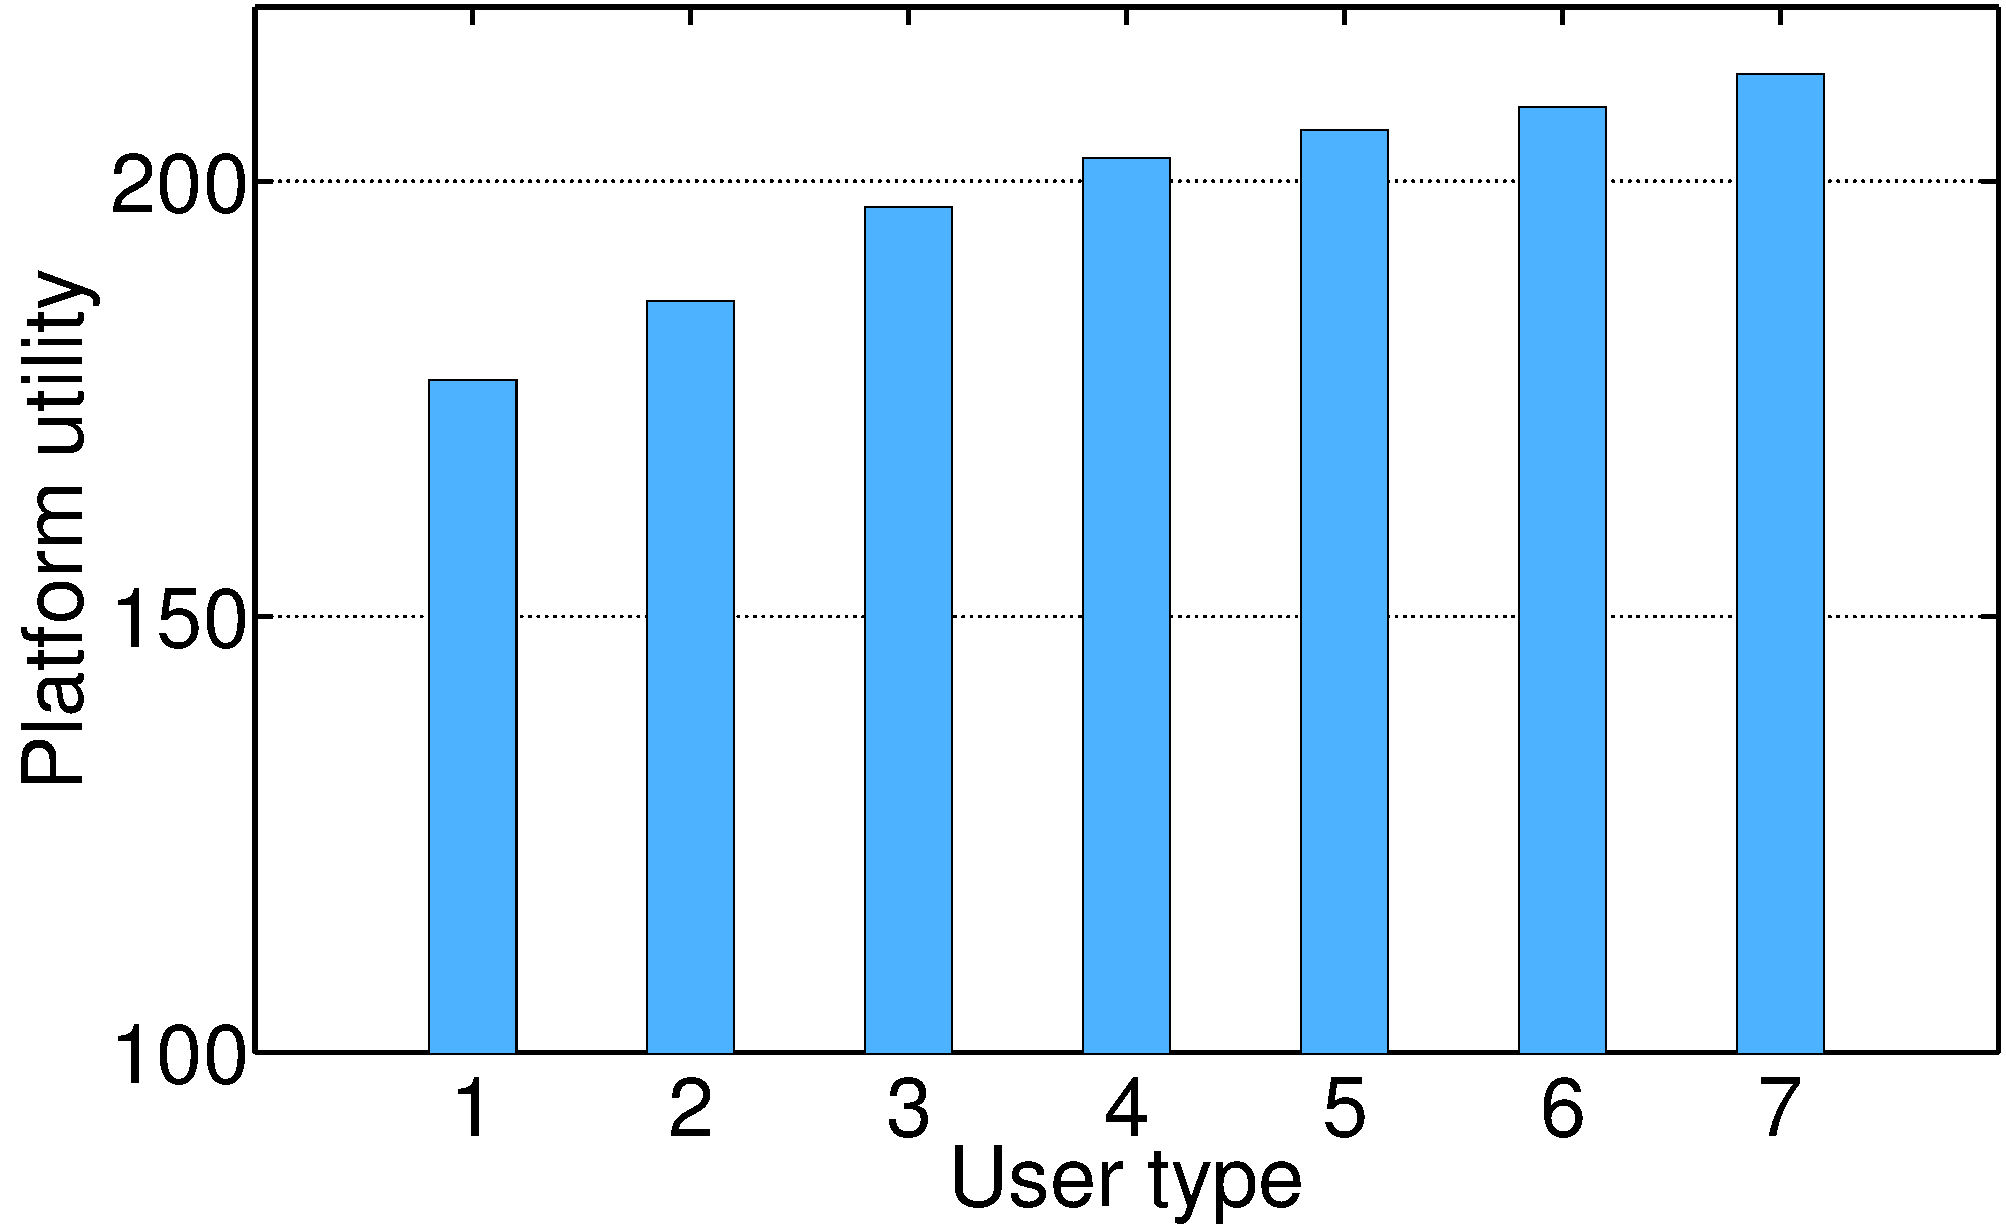
\includegraphics[width=.9\linewidth]{fig3} 
		\caption{Continues figures in landscape mode. (first)}
	\end{figure}

	\begin{figure}[h]
	\centering
	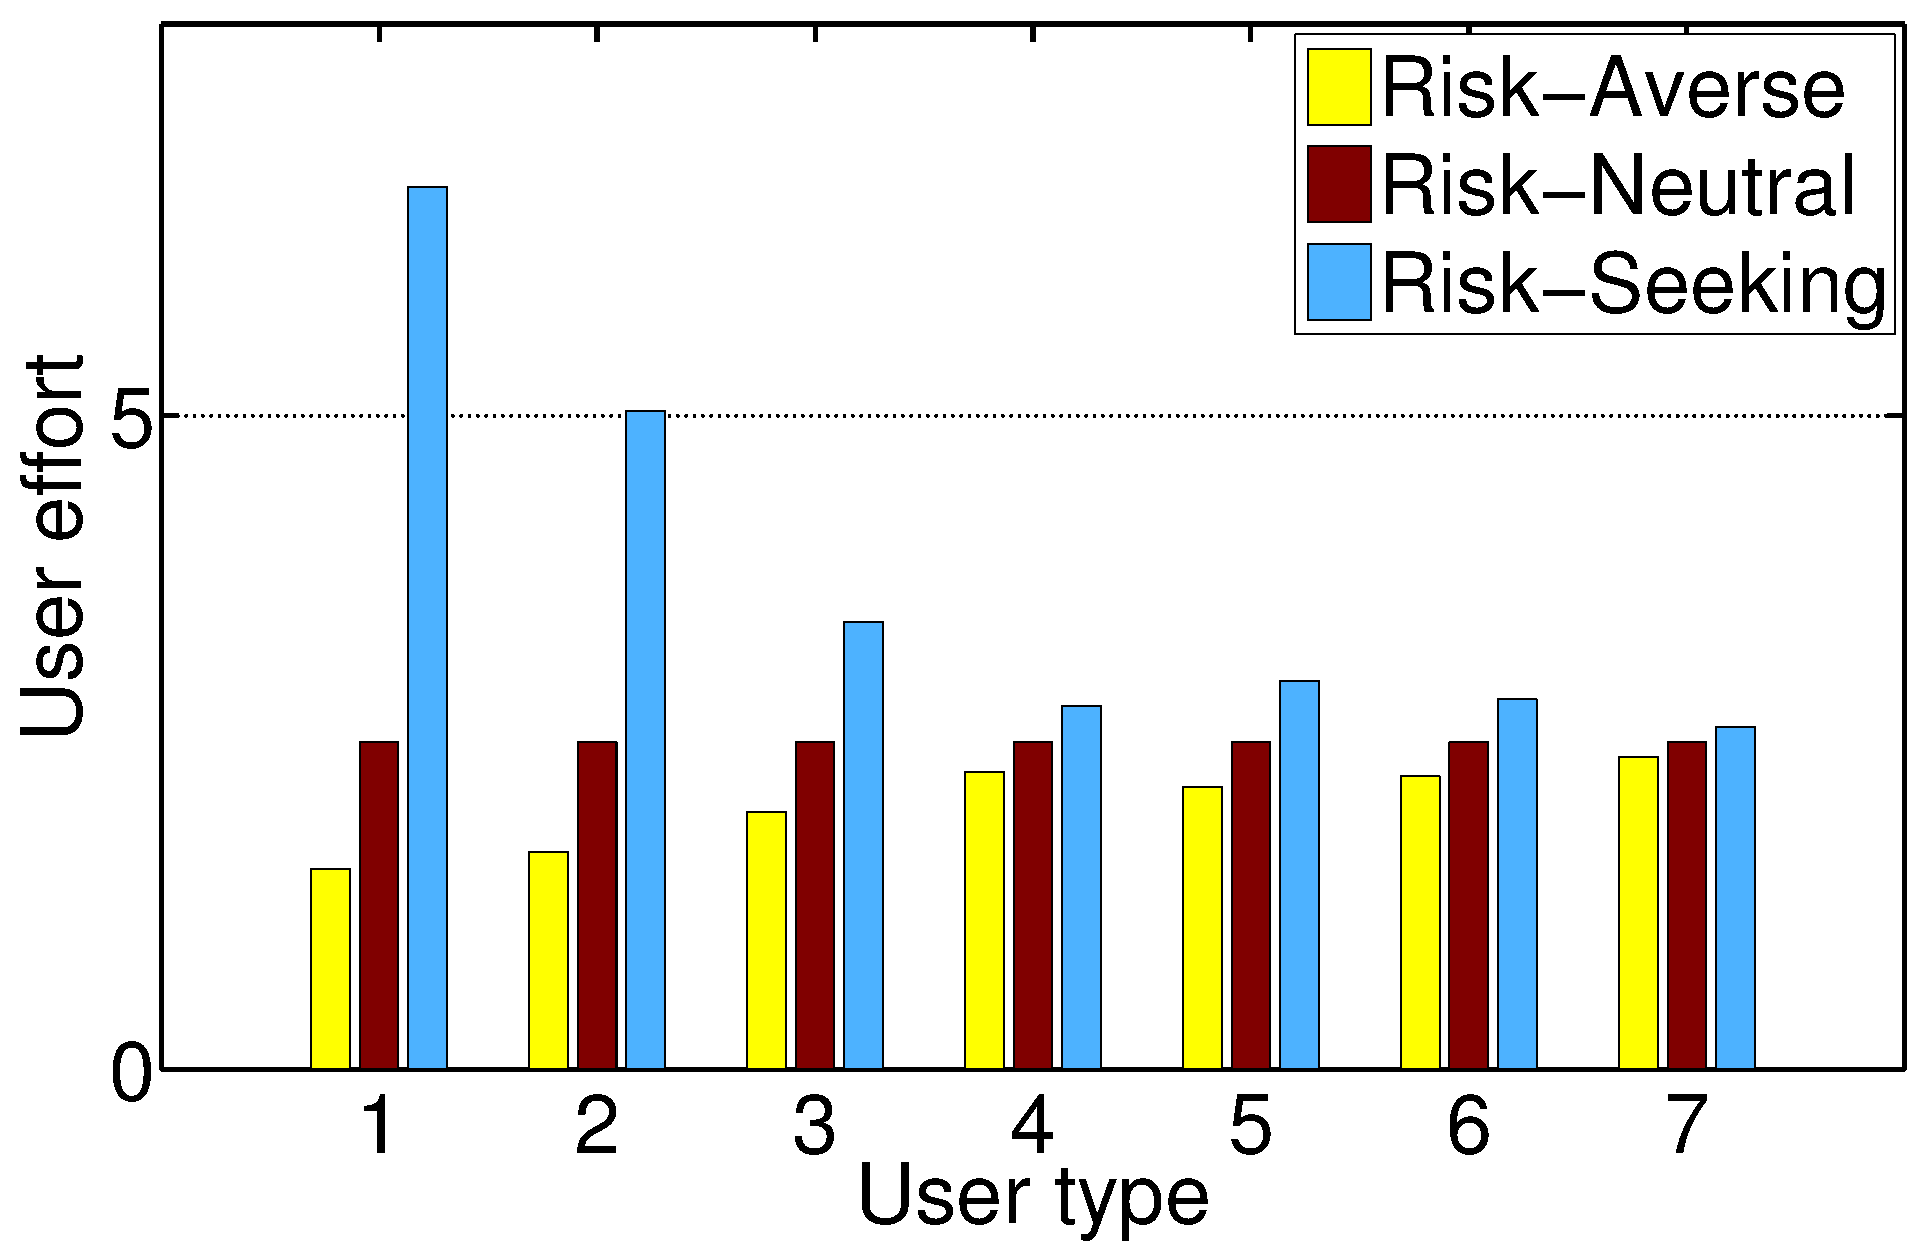
\includegraphics[width=\linewidth]{fig4}
	\caption{Continues figures in landscape mode. (second)}
	\end{figure}
\end{landscape}

Your figures should contain a caption which describes the figure to
the reader. Figure captions go below the figure. Your figures should
{\bfseries also} include a description suitable for screen readers, to
assist the visually-challenged to better understand your work.

Figure captions are placed {\itshape below} the figure.


\begin{landscape} % Require pdflscape and everypage packadge
	\begin{figure}[h]
		\centering
		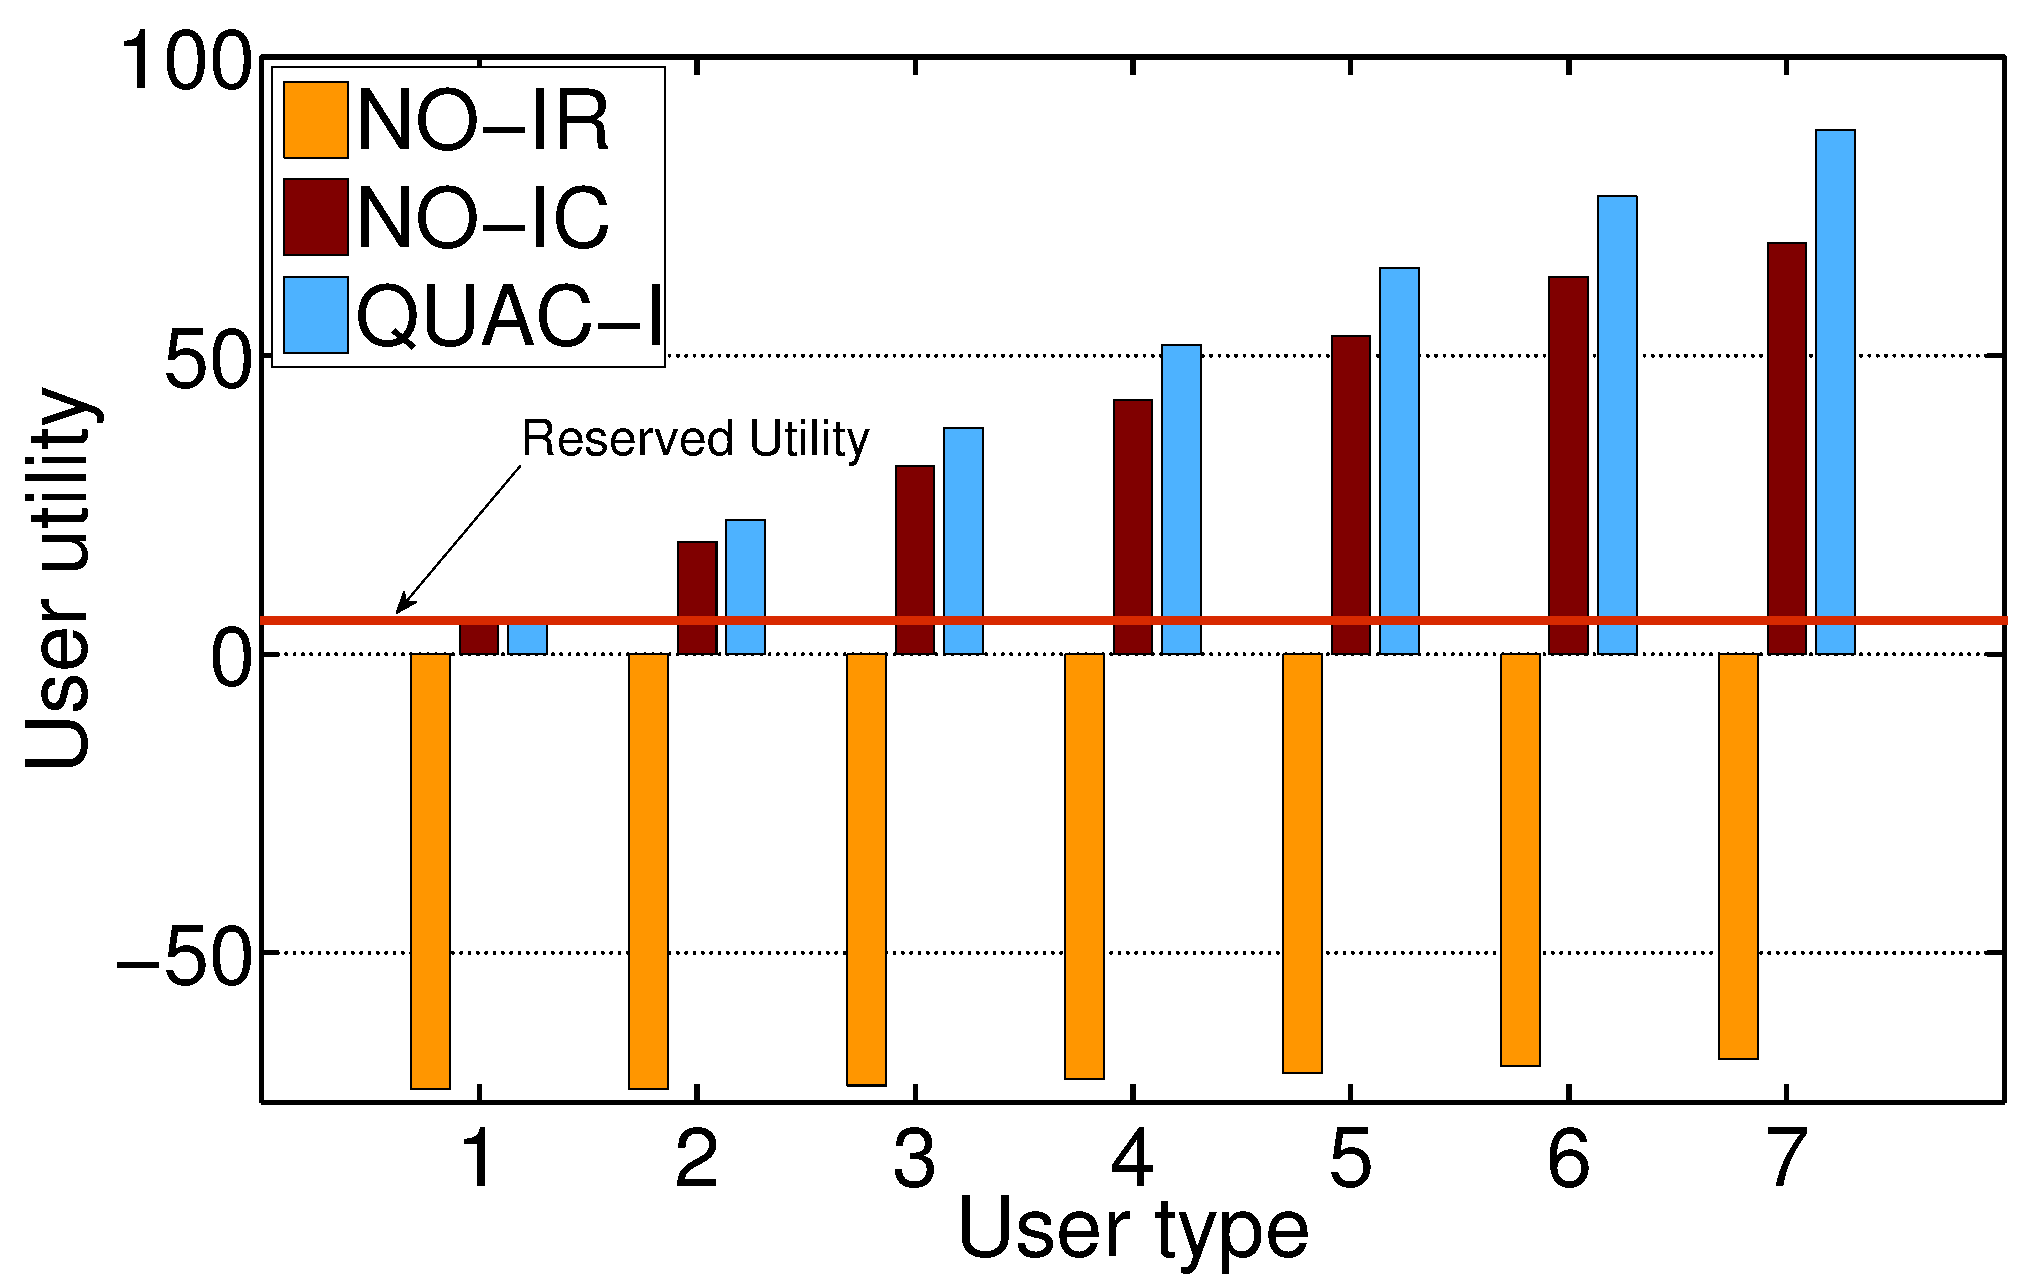
\includegraphics[width=.9\linewidth]{fig6}
		\caption{Example of a figure in landscape mode. Use \texttt{$\backslash$centering} to center the image}
	\end{figure}
\end{landscape}



\begin{figure}[h]
	\centering
	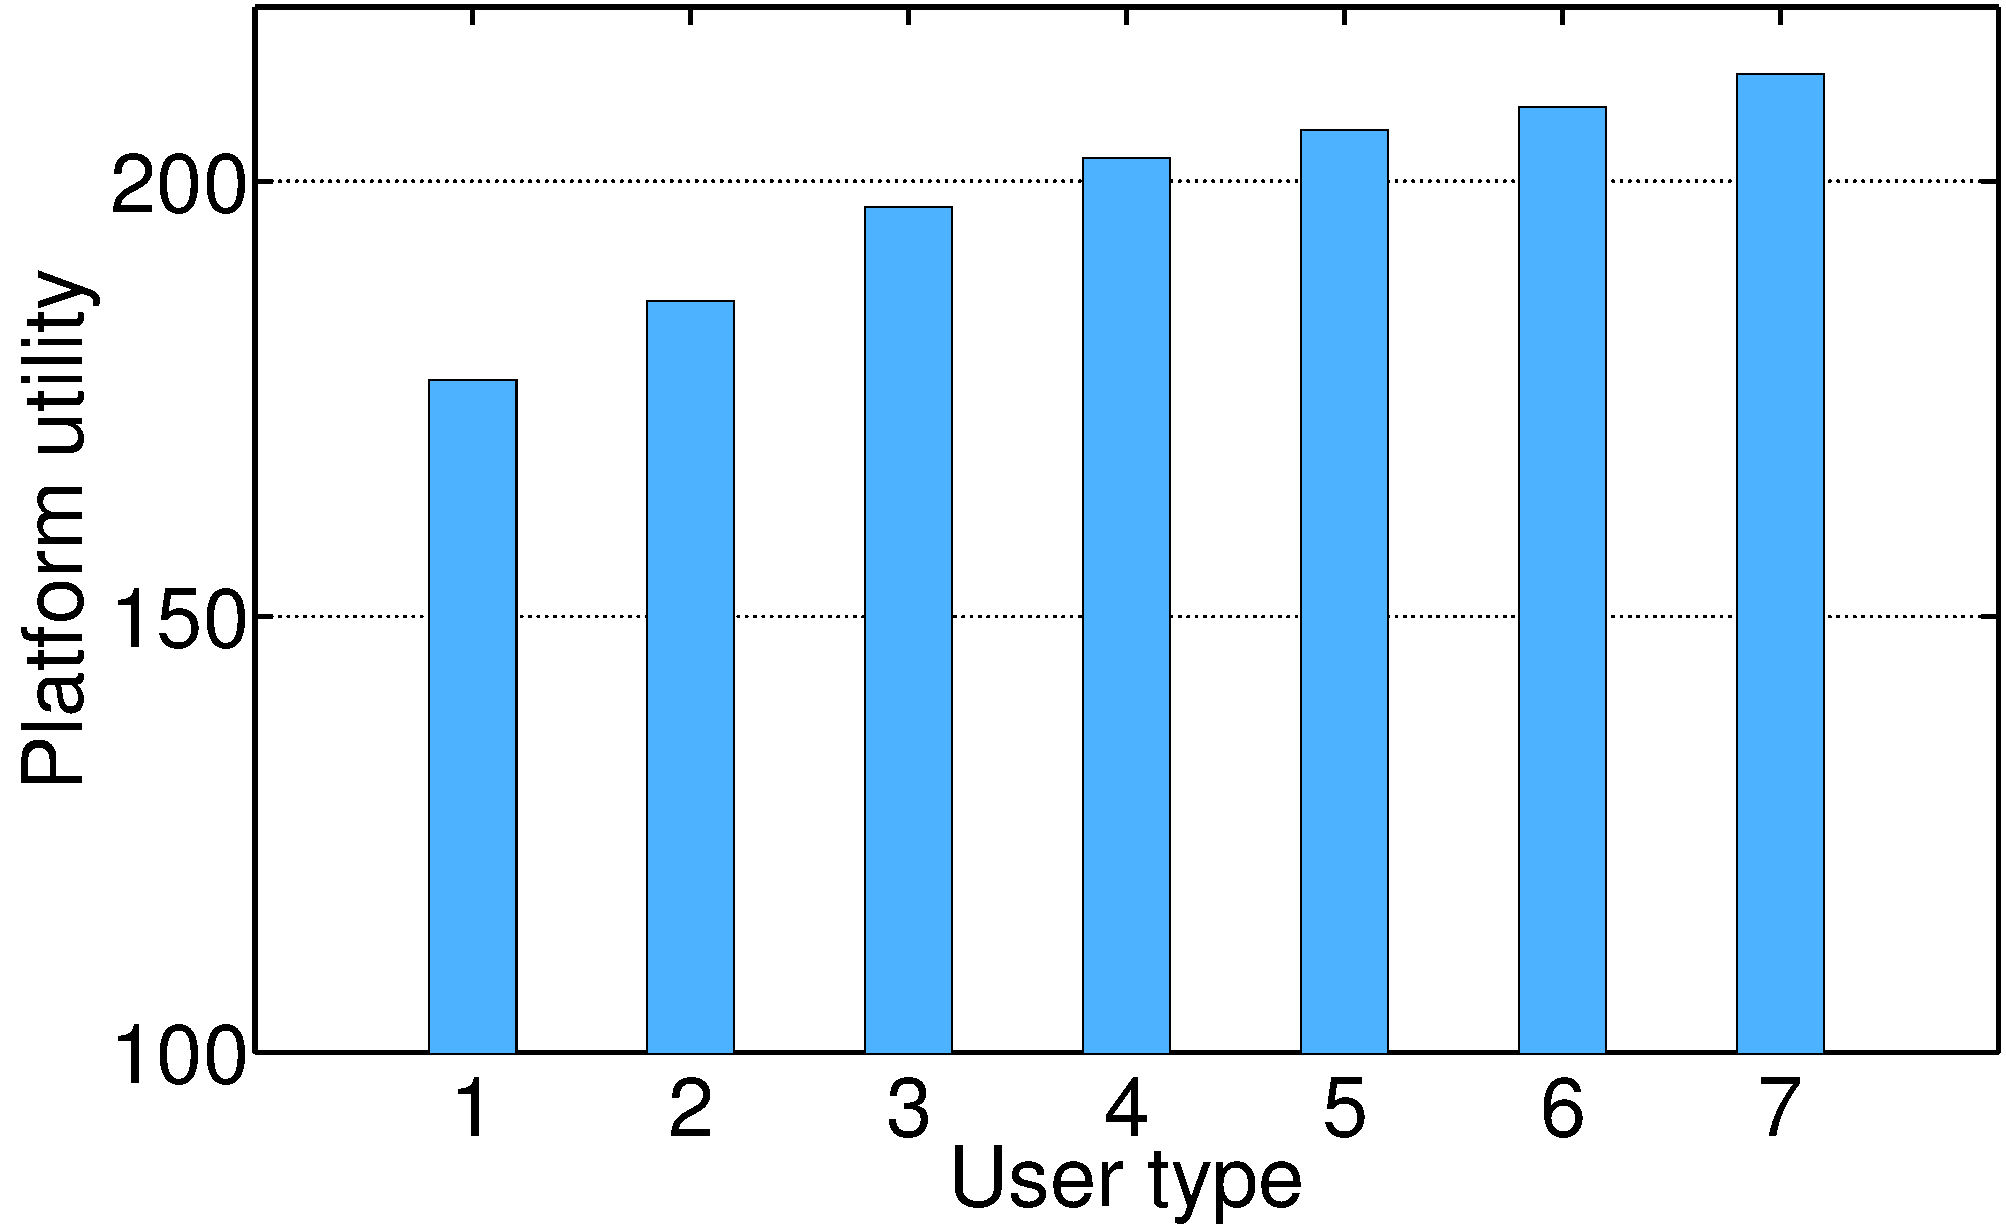
\includegraphics[width=\linewidth]{fig3}
	\caption[Short version caption for LoF, the original caption is really long]{The original realy long long long long long long long long long long long long long long long long long long long long long long long long long long long long long long figure caption.}
\end{figure}
%========================================
%              Section               
%======================================== 
\section{Tables}

The ``\verb|minesthesis|'' document class includes the ``\verb|booktabs|''
package --- \url{https://ctan.org/pkg/booktabs} --- for preparing
high-quality tables.

Table captions are placed {\itshape above} the table.

Because tables cannot be split across pages, the best placement for
them is typically the top of the page nearest their initial cite. To
ensure this proper ``floating'' placement of tables, use the
environment \textbf{table} to enclose the table's contents and the
table caption. The contents of the table itself must go in the
\textbf{tabular} environment, to be aligned properly in rows and
columns, with the desired horizontal and vertical rules. Again,
detailed instructions on \textbf{tabular} material are found in the
\textit{\LaTeX\ User's Guide}.

Immediately following this sentence is the point at which
Table~\ref{tab:freq} is included in the input file; compare the
placement of the table here with the table in the printed output of
this document.

\begin{table}[h]
	\caption{Frequency of Special Characters}
	\label{tab:freq}
	\centering
	\begin{tabular}{ccl}
		\toprule
		Non-English or Math & Frequency   & Comments          \\
		\midrule
		\O                  & 1 in 1,000  & For Swedish names \\
		$\pi$               & 1 in 5      & Common in math    \\
		\$                  & 4 in 5      & Used in business  \\
		$\Psi^2_1$          & 1 in 40,000 & Unexplained usage \\
		\bottomrule
	\end{tabular}
\end{table}


\begin{table*}[h]
	\caption{Some Typical Commands}
	\label{tab:commands}
	\centering
	\begin{tabular}{cclccr}
		\toprule
		Command                    & A Number & Comments         & Command                    & A Number & Comments         \\
		\midrule
		\texttt{{\char'134}author} & 100      & Author           & \texttt{{\char'134}author} & 100      & Author           \\
		\texttt{{\char'134}table}  & 300      & For tables       & \texttt{{\char'134}table}  & 300      & For tables       \\
		\texttt{{\char'134}table*} & 400      & For wider tables & \texttt{{\char'134}table*} & 400      & For wider tables \\
		\bottomrule
	\end{tabular}
\end{table*}

\begin{table*}[h]
	\caption{Some Typical Commands with borders}
	\label{tab:commandswithborders}
	\begin{tabular}{|ccl|ccr|} % use | to add vertical lines
		\hline % use hline instead of toprule/midrule/bottomrule
		Command                    & A Number & Comments         & Command                    & A Number & Comments         \\
		\hline
		\texttt{{\char'134}author} & 100      & Author           & \texttt{{\char'134}author} & 100      & Author           \\
		\texttt{{\char'134}table}  & 300      & For tables       & \texttt{{\char'134}table}  & 300      & For tables       \\
		\texttt{{\char'134}table*} & 400      & For wider tables & \texttt{{\char'134}table*} & 400      & For wider tables \\
		\hline
	\end{tabular}
\end{table*}

\begin{table}[h]
	\caption{Some Typical Commands with borders}
	\label{tab:tabularexample}
	\centering
	\begin{tabular}{>{\ttfamily}m{0.1\textwidth}m{0.2\textwidth}m{0.2\textwidth}} % use | to add vertical lines
		\hline % use hline instead of toprule/midrule/bottomrule
		Command          & A Number & Comments\\
		\hline
		{\char'134}author & 100      & Author            \\
		{\char'134}table & 300      & For tables        \\
		{\char'134}table* & 400      & For wider tables \\
		{\char'134}author & 100      & Author            \\
		{\char'134}table & 300      & For tables        \\
		{\char'134}table* & 400      & For wider tables \\
		\hline
	\end{tabular}
\end{table}



To set a wider table, which takes up the whole width of the page's
live area, use the environment \textbf{table*} to enclose the table's
contents and the table caption. As with a single-column table, this
wide table will ``float'' to a location deemed more
desirable. Immediately following this sentence is the point at which
Table~\ref{tab:commands} is included in the input file; again, it is
instructive to compare the placement of the table here with the table
in the printed output of this document.
\begin{table}[h]
	\caption{Some table with really long long long long long long long long long long long long long long long long long long long long long long long long long long long long long long long long long long long caption}
	\label{tab:commandsnostar}
	\centering
	\begin{tabular}{cclccr}
		\toprule
		Command & A Number & Comments & Command  & A Number & Comments         \\
		\midrule
		\texttt{{\char'134}author} & 100      & Author           & \texttt{{\char'134}author} & 100      & Author           \\
		\texttt{{\char'134}table}  & 300      & For tables       & \texttt{{\char'134}table}  & 300      & For tables       \\
		\texttt{{\char'134}table*} & 400      & For wider tables & \texttt{{\char'134}table*} & 400      & For wider tables \\
		\bottomrule
	\end{tabular}
\end{table}



\begin{landscape}
	\begin{table}[h]
		\caption{A table in landscape mode}
		\label{tab:landscape}
%		\centering
		\begin{tabular}{cclccrlcr}
			\toprule
			Command                    & A Number & Comments         & Command                    & A Number & Comments         & Command                    & A Number & Comments         \\
			\midrule
			\texttt{{\char'134}author} & 100      & Author           & \texttt{{\char'134}author} & 100      & Author           & \texttt{{\char'134}author} & 100      & Author           \\
			\texttt{{\char'134}table}  & 300      & For tables       & \texttt{{\char'134}table}  & 300      & For tables       & \texttt{{\char'134}table}  & 300      & For tables       \\
			\texttt{{\char'134}table*} & 400      & For wider tables & \texttt{{\char'134}table*} & 400      & For wider tables & \texttt{{\char'134}table*} & 400      & For wider tables \\
			\texttt{{\char'134}author} & 100      & Author           & \texttt{{\char'134}author} & 100      & Author           & \texttt{{\char'134}author} & 100      & Author           \\
			\texttt{{\char'134}table}  & 300      & For tables       & \texttt{{\char'134}table}  & 300      & For tables       & \texttt{{\char'134}table}  & 300      & For tables       \\
			\texttt{{\char'134}table*} & 400      & For wider tables & \texttt{{\char'134}table*} & 400      & For wider tables & \texttt{{\char'134}table*} & 400      & For wider tables \\
			\texttt{{\char'134}author} & 100      & Author           & \texttt{{\char'134}author} & 100      & Author           & \texttt{{\char'134}author} & 100      & Author           \\
			\texttt{{\char'134}table}  & 300      & For tables       & \texttt{{\char'134}table}  & 300      & For tables       & \texttt{{\char'134}table}  & 300      & For tables       \\
			\texttt{{\char'134}table*} & 400      & For wider tables & \texttt{{\char'134}table*} & 400      & For wider tables & \texttt{{\char'134}table*} & 400      & For wider tables \\
			\texttt{{\char'134}author} & 100      & Author           & \texttt{{\char'134}author} & 100      & Author           & \texttt{{\char'134}author} & 100      & Author           \\
			\texttt{{\char'134}table}  & 300      & For tables       & \texttt{{\char'134}table}  & 300      & For tables       & \texttt{{\char'134}table}  & 300      & For tables       \\
			\texttt{{\char'134}table*} & 400      & For wider tables & \texttt{{\char'134}table*} & 400      & For wider tables & \texttt{{\char'134}table*} & 400      & For wider tables \\
			\bottomrule
		\end{tabular}
	\end{table}
\end{landscape}



%========================================
%                            Chapter                            
%======================================== 
\chapter{Last chapter}
\lipsum[1]
%========================================
%                            Section                             
%======================================== 
\section{First section} 
\lipsum[2-3]


%========================================
%                            Section                             
%======================================== 
\section{Second section} 
\lipsum[4-5]

%========================================
%                            Section                             
%======================================== 
\section{Last section to test Citation} 

First paper~\cite{goossens1994latex} did something. Note that here we use \verb|~| to make sure the citation not go to the other line. 

Lamport et al.~\cite{lamport1994latex} did something.

Many papers~\cite{makuuchi2000progress,yassin1994latex} did something.


All papers~\cite{makuuchi2000progress,yassin1994latex,
	goossens1994latex,lamport1994latex} did something.

Online link~\cite{onlineWindows} is about something.


% Or add chapters here
\chapter{Last Last chapter}
\lipsum[3]
\section{Section}
\lipsum[4]
\subsection{SubSection} 
\lipsum[4]
\subsubsection{SubSubSection}
\lipsum[4-5]
	
%========================================
%                             Back Matter                               
%========================================
%%================Reference===============
% You may:
% 1. Add one reference section at the end of the thesis/dissertation, 
% or 
% 2. Add a reference section at the end of each chapter
% Set the NAME of your bibliography file
\bibliography{References/referenceAll.bib} 
% Set the STYLE of your reference, you need to compile TWICE
% entries are sorted alphabetically and labelled with numbers.
%\bibliographystyle{plain}
% Chicago style is an "author-date" style, so the citation in the text consists of the author(s) name and year of publication given wholly or partly in round brackets.
\bibliographystyle{chicago}	 % Require natbib package

%%=================Appendix===============
% The \appendix declaration changes the numbering of chapters 
% to an alphabetic form and also changes the names of chapters 
% from \chaptername (default  CHAPTER) to the value 
% of \appendixname (default APPENDIX). 
\appendix 
\chapter{Supplement Data}

Appendix material is information that is not
essential to the text but that contributes to it.

Appendices are used to include information such as the following:

\begin{itemize}
	\item Original data
	\item Long quotations 
	\item Supporting legal decisions or laws 
	\item Computer codes and programs 
	\item Lithologic and petrographic descriptions
	\item Questionnaires 	
	\item Forms and documents 
	\item Permissions to use copyrighted material
	\item Long tables
\end{itemize}


All Figuires and  Tables in an Appendix need to be labeled with a number \& a caption and need to be listed in either the List of Figures or List of Tables.

You may include long appendices as electronic attachments to your thesis. In either instance, appendices are listed in the table of contents.
\chapter{Supplemental Electronic Files}\label{appendix:2}
 The Appendix for the Supplemental Electronic Files should look like the example below. Be sure to include the Appendix in the Table of Contents.
 
 \begin{table}[h]
 	\caption{Example Table in Appendix~\ref{appendix:2}}
 	\label{tab:appendixtable}
 	\centering
 	\begin{tabular}{ccl}
 		\toprule
 		Non-English or Math & Frequency   & Comments          \\
 		\midrule
 		\O                  & 1 in 1,000  & For Swedish names \\
 		$\pi$               & 1 in 5      & Common in math    \\
 		\$                  & 4 in 5      & Used in business  \\
 		$\Psi^2_1$          & 1 in 40,000 & Unexplained usage \\
 		\bottomrule
 	\end{tabular}
 \end{table}

\end{document}